%!TeX root = main.tex
%!encoding = UTF-8 Unicode

\subsection{Verification}
This section verifies the performance of the dual-channel differential active voltage probe and establishes the limits of its use in switching measurements.
Because the high-pass channel targets drain-source voltage components that are difficult to resolve with conventional probes, independent reference measurements are required to assess its accuracy.
The tests address the relevant error mechanisms introduced in Section~\ref{sec:fundamental_measurement_errors}, including limited bandwidth, large-signal distortion, parasitic coupling, and noise.
Together, these tests establish the conditions under which the subsequent analysis of device behavior can be interpreted.

The verification proceeds from controlled reference measurements to tests in the intended switching environment.
A vector network analyzer (VNA) first characterizes the small-signal frequency response of both channels.
A resistively loaded \SI{50}{\ohm} pulse generator and the associated verification methodology were developed in this work and presented in~\cite{kragl_active_2025}.
Beyond verifying the overall large-signal response, the pulse generator enables independent verification of small high-frequency voltage components.
Switching measurements then assess parasitic coupling, common-mode errors, and shielding effectiveness.
The final noise characterization identifies the mechanisms that limit the usable measurement range.









\subsubsection*{Small-Signal Verification}
The small-signal verification determines the frequency response and input-path symmetry of both channels.
The VNA magnitude measurements assess the low-pass gain flatness and the usable frequency range of both channels.
The design targets are a bandwidth exceeding \SI{120}{MHz} for the low-pass channel and \SI{500}{MHz} for the high-pass channel.
The low-pass target covers the range in which conventional switching measurements typically remain above the noise floor.
Assessing these targets requires separate measurements of the two differential input paths.

The available two-port VNA requires the differential probe to be measured in two single-ended configurations.
The VNA was calibrated at the probe input using an Open-Short-Load procedure with a \SI{50}{\Omega} source impedance.
As shown in \fref{fig:EME_VNA_SchematicOverview}, the shared ground of the two VNA ports shorts on side of probe (either positive or negative).
Swapping the positive and negative input connections therefore yields the response of each path separately.
Comparing these responses assesses the input-path symmetry needed for common-mode rejection.

\begin{figure}[ht]
	\centering
	\import{./figures/4_VoltageProbe/}{Diss_SchematicOverview_EME_VNA.pdf_tex}
	\caption{Small-signal verification setup: single-ended VNA measurement of one differential input at a time. The VNA ground connection shorts the inactive differential input; the measurement is repeated with swapped connections to characterize both input paths.}\label{fig:EME_VNA_SchematicOverview}
\end{figure}

The VNA results show the responses of both input paths for each output channel.
The positive and negative paths are plotted as solid and dashed lines in \fref{fig:VNA_LP} and \fref{fig:VNA_HP}, respectively.
The source power was \SI{0}{dBm} for the positive input and \SI{-10}{dBm} for the negative input.
The corresponding noise floors in \mti{S}{11,LP} are approximately \SI{-100}{dB} and \SI{-80}{dB}, respectively.

\begin{figure}[ht]
	\centering
	\input{"figures/4_VoltageProbe/VNA_LP.tex"}
	\caption{VNA measurement of positive (LPp) and negative (LPn) low-pass paths, crosscheck~\fref{fig:EME_VNA_SchematicOverview}.}\label{fig:VNA_LP}
\end{figure}

The measured S-parameters also determine the probe voltage gain \mti{a}{probe}.
The input reflection coefficient accounts for the voltage at the probe input, giving
\begin{align}
	\mti{a}{probe} 	&= \frac{\mi{v}{out}}{\mi{v}{HV+}-\mi{v}{HV-}} \\
					&= \frac{\mti{S}{21}}{1 + \mti{S}{11}}.
\label{eq:TF_probe}
\end{align}

Since \mti{S}{11} remains nearly constant because of the high input impedance, \mti{S}{21} determines most of the frequency dependence of the gain.
Applying this single-ended equation to differential measurements assumes equal gains in both input paths.
A gain mismatch makes the output depend additionally on the common-mode voltage relative to oscilloscope ground.



The low-pass channel exceeds its bandwidth target and shows close agreement between the input paths.
Its flat passband gain of \SI{-53}{dB} corresponds to a voltage division ratio of 446, close to the divider design value.
The \SI{3}{dB} bandwidth is \SI{315}{MHz} and is primarily limited by the low-pass subtractor operational amplifier (see \fref{fig:VNA_rawLP}).
The maximum input-path gain deviation is \SI{0.2}{dB} at \SI{3}{MHz}.
These results support differential measurements up to and beyond the \SI{120}{MHz} design target.

The high-pass channel provides the intended rising response, but input-path agreement deteriorates near the upper frequency limit.
As shown in \fref{fig:VNA_HP}, the magnitude slope is approximately \SI{+40}{dB/dec} from \SI{1}{MHz} to \SI{450}{MHz}, beyond which the unity-gain output amplifier begins to roll off, compare \fref{fig:VNA_rawUG}.
The input-path gain deviation remains below \SI{0.8}{dB} in this rising region.
The deviation increases to \SI{2.8}{dB} at \SI{490}{MHz} as the paths approach their respective roll-off frequencies.
The measured \SI{3}{dB} bandwidth exceeds \SI{400}{MHz}, but the growing mismatch limits common-mode rejection near the \SI{500}{MHz} target.

\begin{figure}[ht]
	\centering
	\input{"figures/4_VoltageProbe/VNA_HP.tex"}
	\caption{VNA measurement of positive (HPp) and negative (HPn) high-pass paths, crosscheck~\fref{fig:EME_VNA_SchematicOverview}.}\label{fig:VNA_HP}
\end{figure}

The remaining S-parameters characterize the probe interfaces and residual reverse coupling.
Both channel measurements show a voltage-divider feature at \SI{695}{MHz}.
The output reflection coefficient \mti{S}{22} is consistent with the specified \SI{10}{\Omega} output resistance.
The input reflection coefficient \mti{S}{11} is approximately \SI{0}{dB}, consistent with the high input impedance of the divider.
The reverse transmission \mti{S}{12} reveals residual passive coupling from output to input.
These measurements describe the small-signal behavior; the following pulse-generator tests assess performance at switching-voltage amplitudes.













\subsubsection*{Large-Signal Verification}
The large-signal verification tests whether the probe preserves both the switching waveform and its small high-frequency components at high input voltage.
Small-signal VNA measurements alone cannot establish this performance because amplifier distortion depends on signal amplitude.
The reference source is the \SI{400}{V}, \SI{50}{\ohm} pulse generator developed for this purpose.
Its resistive load allows a reference measurement independent of the voltage probe, as shown in \fref{fig:MS_PulsGen_ESB}.

\begin{figure}[ht]
	\centering
	\import{./figures/4_VoltageProbe/}{Diss_PulseGenerator_ESB.pdf_tex}
	\caption{Large-signal verification of the low-pass and high-pass channels using a \SI{50}{\ohm} pulse generator~\cite{kragl_active_2025}. The reference is acquired both via a conventional direct measurement and through a commercial \SI{180}{MHz}--\SI{340}{MHz} passive band-pass filter.}\label{fig:MS_PulsGen_ESB}
\end{figure}

The pulse-generator setup provides a directly measurable reference for the switching voltage.
A \SI{40}{dB} attenuator serves as the \SI{50}{\Omega} load and permits direct connection to the oscilloscope.
The oscilloscope bandwidth is \SI{2}{GHz}.
The physical arrangement is shown in \fref{fig:MS_PulsGen_Pic}.
The reference can therefore be acquired without an additional high-voltage probe.

\begin{figure}[ht]
	\centering
	\import{./figures/4_VoltageProbe/}{Diss_PulseGenerator_Pic.pdf_tex}
	\caption{Large-signal verification of the low-pass and high-pass channels using a \SI{50}{\ohm} pulse generator~\cite{kragl_active_2025}. The reference is acquired both via a conventional direct measurement and through a commercial \SI{180}{MHz}--\SI{340}{MHz} passive band-pass filter.}\label{fig:MS_PulsGen_Pic}
\end{figure}

The pulse generator produces fast transitions for testing the probe's large-signal response.
It uses \SI{750}{V} GaN-HEMTs to switch the resistive load, producing rise times below \SI{10}{ns}.
These transitions expose amplitude-dependent limitations that are not captured by the VNA measurement.
The \SI{50}{\Omega} interface also accepts commercial BNC band-pass filters, thereby filtering the frequency range of interest and diminishing the problem of quantization noise.
The setup thus supports both time-domain verification of the switching edge and frequency-domain verification of small high-frequency components.


The low-pass channel captures the initial switching edge but exhibits a distorted settling response.
\fref{fig:MS_PulsGen_TD} compares the DAVP low-pass output with the attenuated pulse-generator reference and a commercial passive high-voltage probe.
The initial rising edge agrees with the reference, whereas the transient tail shows second-order (PT2) behavior.
The output settles to its final value after approximately \SI{20}{ns}.
The small-signal bandwidth of \SI{315}{MHz} therefore does not fully describe the low-pass channel's transient accuracy.

The settling distortion is attributed to the amplitude-dependent response of the low-pass subtractor amplifier.
According to its datasheet, the bandwidth decreases from \SI{800}{MHz} at \SI{100}{mVpp} to \SI{250}{MHz} at \SI{2}{Vpp} and \SI{140}{MHz} at \SI{4}{Vpp}.
The shared unity-gain buffer retains measured bandwidths of \SI{3.1}{GHz} at \SI{100}{mVpp} and \SI{1.6}{GHz} at \SI{2}{Vpp}.
The observed distortion is thus associated with the low-pass subtractor rather than the shared buffer.
The separate high-pass path is assessed using a band-limited reference measurement.


\begin{figure}[ht]
	\centering
	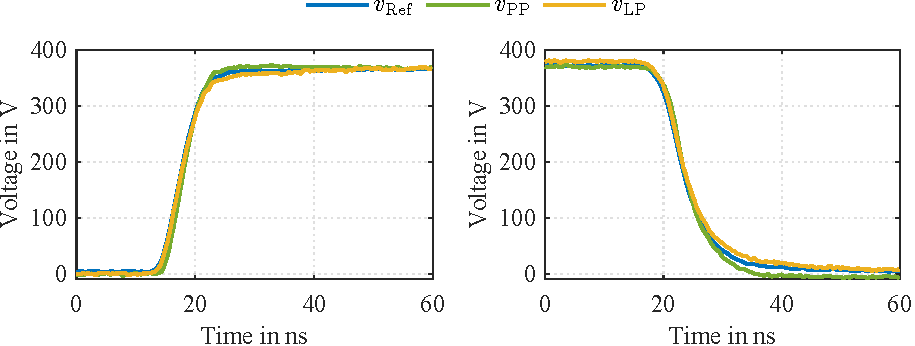
\includegraphics[scale=1]{figures/4_VoltageProbe/MS_PulsGen_TD.pdf}
	\caption{Large-signal verification time-domain of the low-pass using a \SI{50}{\ohm} pulse generator~\cite{kragl_active_2025}. The reference is acquired both via a conventional direct measurement and through a commercial \SI{180}{MHz}--\SI{340}{MHz} passive band-pass filter.}\label{fig:MS_PulsGen_TD}
\end{figure}

The high-pass channel is verified against a band-pass-filtered reference that isolates the small high-frequency voltage components.
A commercial passive BNC filter passes \SIrange{180}{340}{MHz} while attenuating the dominant DC and low-frequency content.
The filter and the high-pass channel have different time-domain responses, so the comparison uses calibrated frequency-domain results.
\fref{fig:MS_PulsGen_Meas} compares the unfiltered reference, the filtered reference, and both DAVP channels.
A pulse sequence is used to obtain comparable quantization-noise floors in the reference and measurement channels.
The resulting spectra allow the high-pass amplitude accuracy to be assessed within the reference passband.

\begin{figure}[ht]
	\centering
	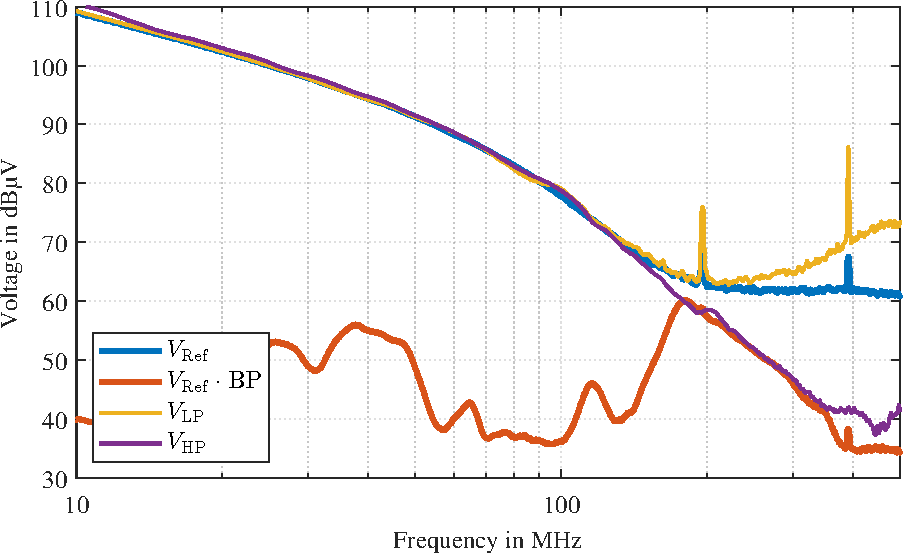
\includegraphics[scale=1]{figures/4_VoltageProbe/MS_PulsGen.pdf}
	\caption{Large-signal verification of the low-pass and high-pass channels using a \SI{50}{\ohm} pulse generator~\cite{kragl_active_2025}. The reference is acquired both via a conventional direct measurement and through a commercial \SI{180}{MHz}--\SI{340}{MHz} passive band-pass filter.}\label{fig:MS_PulsGen_Meas}
\end{figure}

The high-pass channel agrees with the independent reference within the band-pass filter's passband.
Across \SIrange{180}{340}{MHz}, the maximum deviation is \SI{1.3}{dB} at \SI{200}{MHz}.
The deviation remains below \SI{1}{dB} across most of that band.
Agreement with the unfiltered reference and the low-pass channel is also observed where those spectra remain above their noise floors.
Below \SI{10}{MHz}, the high-pass deviation increases as the signal is increasingly attenuated.
The band-pass comparison therefore provides the independent evidence for resolving small high-frequency components under large-signal excitation.

Independent large-signal verification is limited to \SI{340}{MHz} by the available reference filter.
No suitable commercial band-pass filter extending the reference measurement through the \SIrange{300}{400}{MHz} region was available for this setup.
Above \SI{340}{MHz}, the measured spectrum forms a plateau rather than the expected continuous roll-off.
This feature indicates a possible measurement artifact, so the \SI{1.3}{dB} deviation cannot be extended to that range.
For the rest of this work, results are presented up to \SI{500}{MHz}, but values above \SI{340}{MHz} have to be interpreted as comparative rather than independently verified absolute values.

The pulse-generator measurements establish different limits for the two channels.
The low-pass channel resolves the initial edge but requires approximately \SI{20}{ns} to settle.
The high-pass channel resolves the small components in the independent reference band with a maximum deviation of \SI{1.3}{dB}.
These controlled tests do not reproduce all coupling paths of a commutation cell, which are assessed next under switching conditions.











\subsubsection*{Parasitic Coupling and Common-Mode Error}

The switching tests assess errors caused by the probe's interaction with the intended application environment.
Parasitic coupling and common-mode feedthrough can distort the drain-source voltage even when the differential response agrees with a controlled reference.
The DAVP and a commercial passive probe therefore measure a SiC MOSFET in the commutation cell used later in this work.
The cell operates in double-pulse test with the actively switched device in the low-side position.
This arrangement permits a waveform comparison and a separate common-mode error measurement under the relevant switching conditions.

The passive-probe comparison and the common-mode test address different error contributions.
The waveform comparison is primarily performed in the time domain because quantization noise limits the passive reference at high frequencies.
For the common-mode test, both DAVP inputs are connected to the MOSFET source terminal.
With no applied differential voltage, the remaining output measures the residual error under common-mode excitation.
The results in \fref{fig:Voltage_DPT_LPvsPP_weCM_TD} and \fref{fig:Voltage_DPT_HPvsPP_weCM_TD} must therefore be interpreted according to the purpose of each test.

\begin{figure}[ht]
	\centering
	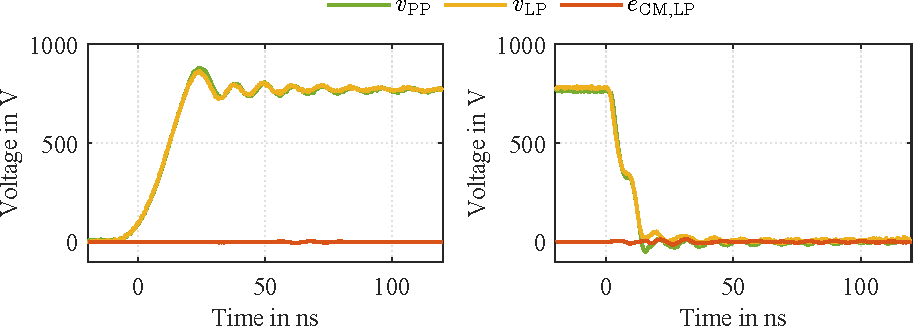
\includegraphics[scale=1]{figures/4_VoltageProbe/Voltage_DPT_LPvsPP_weCM_TD.pdf}
	\caption{Time-domain measurement results of PMTX05, at 800V, 30A room temperature, cross validation of passive probe and low-pass measurement to crosscheck inductive and capacitive coupling effects.}\label{fig:Voltage_DPT_LPvsPP_weCM_TD}
\end{figure}

The low-pass waveform agrees closely with the passive reference under switching conditions.
The remaining deviation is consistent with the previously observed large-signal settling limitation.
The settling interval is approximately \SI{14}{ns} during active-on and \SI{32}{ns} during active-off switching.
The comparison does not reveal additional coupling that materially changes the overall waveform, but it does not independently verify the small high-frequency components of the high-pass measurement.

The dedicated common-mode test quantifies the residual error that is not separated by the waveform comparison.
The error remains below \SI{4}{V} during active-off and below \SI{14}{V} during active-on switching.
These values correspond to less than \SI{1.8}{\percent} of the measured voltage.
Common-mode feedthrough is therefore small relative to the overall switching-voltage amplitude, although that ratio alone does not establish its significance for small high-frequency components.

The high-pass measurements provide a corresponding time-domain check of residual common-mode errors.
\fref{fig:Voltage_DPT_HPvsPP_weCM_TD} shows the differential response and the output under common-mode excitation.

\begin{figure}[ht]
	\centering
	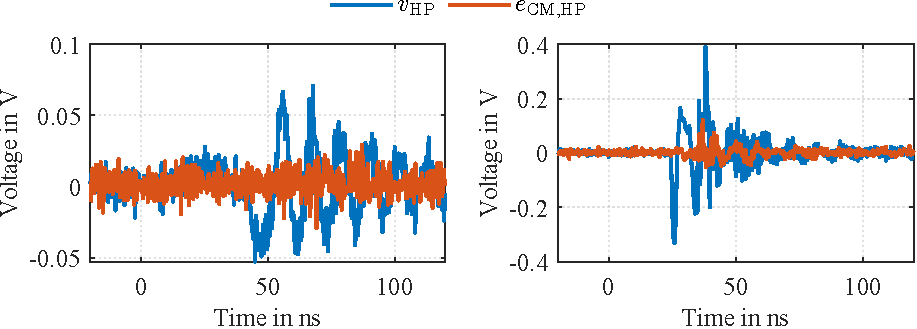
\includegraphics[scale=1]{figures/4_VoltageProbe/Voltage_DPT_HPvsPP_weCM_TD.pdf}
	\caption{Time-domain measurement results of PMTX05, at 800V, 30A room temperature, cross validation of passive probe and high-pass measurement to crosscheck inductive and capacitive coupling effects.}\label{fig:Voltage_DPT_HPvsPP_weCM_TD}
\end{figure}

To highlight the influence of parasitic coupling, a test with and without shielding is conducted, as shown in \fref{fig:Influence_Shield_TD} and \fref{fig:Influence_Shield_FD}.
Without shielding, the time-domain waveform exhibits greater overshoot and ringing.
The corresponding spectrum also shows higher amplitudes at high frequencies.
These differences support the use of the shield to reduce environmental coupling.

Shielding reduces the observed interference but does not eliminate all residual waveform deviations.
Small oscillations and an offset remain while the MOSFET is on.

\begin{figure}[ht]
	\centering
	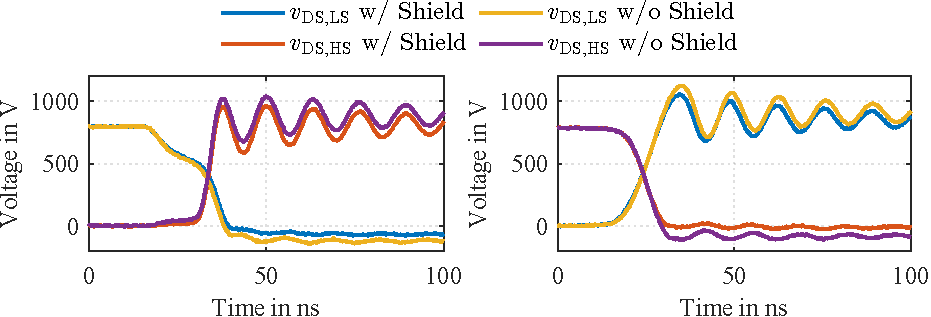
\includegraphics[scale=1]{figures/4_VoltageProbe/Influence_Shield_TD.pdf}
	\caption{Time-domain measurement results of PMTX05, at 800V, 30A room temperature, influence of the shield on the measurement.}\label{fig:Influence_Shield_TD}
\end{figure}

\begin{figure}[ht]
	\centering
	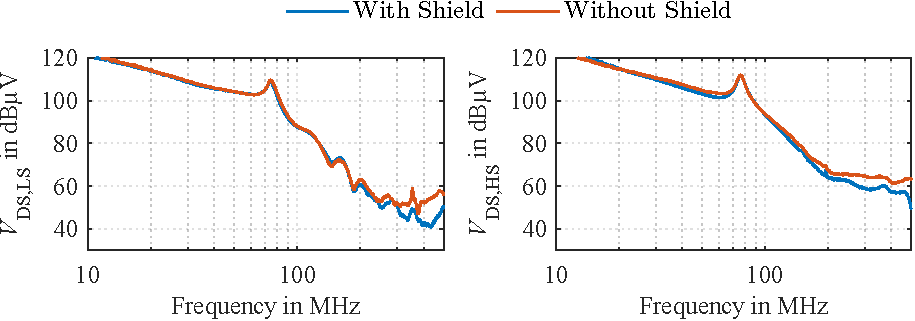
\includegraphics[scale=1]{figures/4_VoltageProbe/Influence_Shield_FD.pdf}
	\caption{Frequency-domain measurement results of PMTX05, at 800V, 30A room temperature, influence of the shield on the measurement.}\label{fig:Influence_Shield_FD}
\end{figure}


\subsubsection*{Noise Performance Characterization}
The noise characterization determines which noise sources limit the resolution of small voltage components.
Unlike the preceding reference comparisons, this analysis does not directly verify signal accuracy.
Measurements with and without the probe separate its contribution from the oscilloscope noise, while different acquisition ranges expose the quantization-noise contribution.
The results establish the noise limits needed to interpret the subsequent device measurements.


Four acquisition configurations separate probe noise from oscilloscope noise.
The acquisition length is \SI{5}{ms}, matching the pulse-chain duration used later.
\fref{fig:Diss_Voltage_NoiseContribution} first compares measurements at the vertical resolution used for the switching signals, with the probe connected (Probe + HV Resolution) and disconnected (HV Resolution).
The measurements are then repeated with full ADC resolution, again with the probe connected (Probe + Full Resolution) and disconnected (Full Resolution).
Comparing these configurations identifies the noise contribution that dominates in each frequency range.

\begin{figure}[hbt]
	\centering
	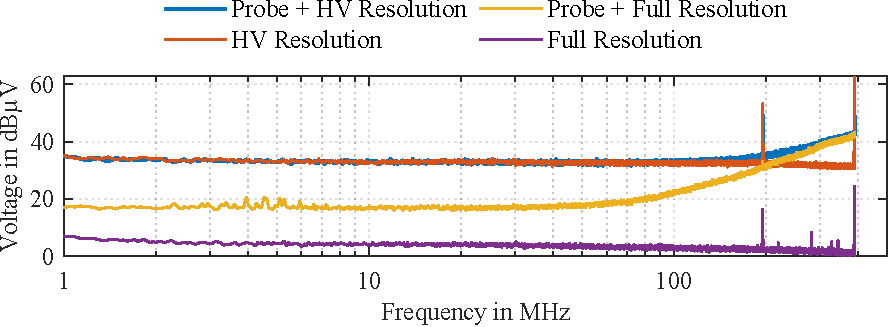
\includegraphics[scale=1]{figures/4_VoltageProbe/Diss_Voltage_NoiseContribution.pdf}
	\caption{Frequency domain measurement of the noise limiting effects of the EME voltage probe.}\label{fig:Diss_Voltage_NoiseContribution}
\end{figure}

Quantization noise limits the oscilloscope measurement at the acquisition range used for the switching signals.
Without the probe, using full ADC resolution reduces the measured noise level from \SI{50}{dBµV} to \SI{22}{dBµV}.
With the probe connected, its intrinsic noise remains below the HV-resolution quantization-noise level of \SI{33}{dBµV} up to approximately \SI{100}{MHz}.
The probe contribution then rises with frequency and exceeds the quantization-noise contribution at approximately \SI{200}{MHz}.
Intrinsic probe noise therefore limits the measurement at higher frequencies, even when quantization noise is reduced.

Discrete spectral peaks reveal an additional oscilloscope contribution that is distinct from the broadband noise floor.
The peaks occur at \SI{196}{MHz} and its harmonics, corresponding to the oscilloscope's ADC interleaving frequency.
Interleaving combines time-offset samples from several ADCs to increase the effective sampling rate.
Mismatch between the ADCs can introduce periodic errors and corresponding spectral components.
These peaks must therefore be distinguished from both intrinsic probe noise and device-related spectral features.

\begin{figure}[hbt]
	\centering
	\import{./figures/4_VoltageProbe/}{Diss_Highpass_EME_NoiseSources_ESB.pdf_tex}
	\caption{Equivalent circuit diagram of the noise sources for the first high-pass amplification stage.}\label{fig:ESB_OP_noiseSources}
\end{figure}

An analytical calculation of the second high-pass amplification stage explains the frequency dependence of the intrinsic probe noise.
\fref{fig:ESB_OP_noiseSources} shows the noise-source model of a high-pass stage, where \mi{Z}{g} represents the series capacitor and resistor network.
Each resistor contributes Johnson--Nyquist thermal noise.
The ideal capacitor generates no thermal noise; a real capacitor contributes through its equivalent series resistance (ESR).
The operational amplifier adds input voltage noise and input current noise.
The calculation therefore includes the following contributions:
\begin{itemize}
	\item incoming noise from preceding stages,
	\item amplifier input voltage noise,
	\item resistor thermal noise,
	\item amplifier input current noise.
\end{itemize}

The resistor thermal noise is given by
\begin{equation}
	\mi{V}{n,th} = \sqrt{4\mi{k}{B}TR\Delta f}.
\end{equation}

The effective noise gain of the high-pass stage is
\begin{equation}
	 NG = 1 + \frac{\mi{R}{f}}{\mi{Z}{g}}.
\end{equation}

The total output noise can then be expressed as
\begin{equation}
	\mi{v}{0} = \sqrt{(\mi{v}{n,in} NG)^2 + (\mi{v}{n} NG)^2 + 2(\mi{i}{n} \mi{R}{f})^2 + 2\cdot4\mi{k}{B}T\mi{R}{f}\Delta f + 2\cdot4\mi{k}{B}T\mi{R}{g}\Delta f \left(\frac{\mi{R}{f}}{\mi{Z}{g}}\right)^2}.
\end{equation}

The frequency-dependent noise gain shapes the amplifier's output-noise contribution.
The expression combines amplifier noise, resistor noise, and noise arriving from the preceding stage.
The resulting contributions can be compared to identify the source of the measured high-frequency noise rise.

The calculated contributions identify amplifier noise as the main intrinsic limitation.
Using datasheet values, \fref{fig:Diss_Voltage_NoiseCalc} shows that input current noise dominates at low frequencies and input voltage noise dominates at higher frequencies.
Resistor thermal noise contributes little for the selected resistance values of a few hundred \si{\ohm}.
Noise from the preceding stage also increases with frequency as it propagates through the cascade.
The calculated response changes from first- to second-order behavior near \SI{100}{MHz}.
The calculation thus explains why the intrinsic noise contribution rises toward the upper measurement range.


\begin{figure}[hbt]
	\centering
	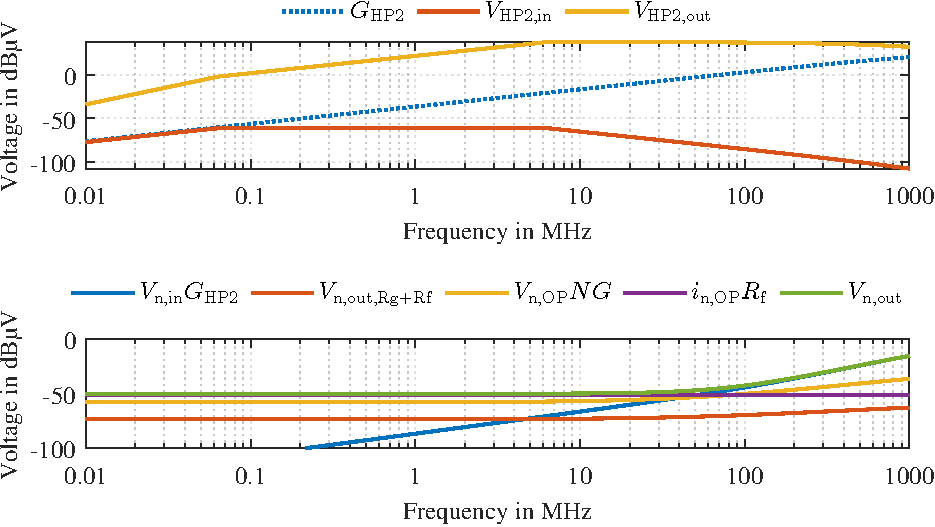
\includegraphics[scale=1]{figures/4_VoltageProbe/Diss_Voltage_Calc_Noise.pdf}
	\caption{Calculation of the noise sources for the first high-pass amplification stage.}\label{fig:Diss_Voltage_NoiseCalc}
\end{figure}



\subsubsection*{Verification Summary and Measurement Limits}
The verification establishes a usable measurement range that depends on both frequency and signal amplitude.
The low-pass channel has a small-signal bandwidth of \SI{315}{MHz}, but its large-signal settling response limits the accuracy of the transient tail.
The pulse-generator method independently verifies small high-frequency components within \SIrange{180}{340}{MHz}, with a maximum observed deviation of \SI{1.3}{dB}.
Measurements above \SI{340}{MHz} remain comparative rather than independently verified absolute results.

The application measurements must also account for residual common-mode errors, environmental coupling, and noise.
The switching tests show close low-pass agreement with a passive reference and reduced interference with shielding, but neither result establishes an error-free high-frequency measurement.
Intrinsic probe noise becomes dominant above approximately \SI{200}{MHz}, and ADC interleaving adds discrete spectral peaks.
Subsequent device comparisons are therefore interpreted within these verification and noise limits.